% ------------------------------------------------------------
%  Módulo de medición de temperatura: cuatro sensores DS18B20
%  sobre buses 1-Wire independientes.
% ------------------------------------------------------------
\begin{figure}[H]
  \centering
  \resizebox{\textwidth}{!}{%
  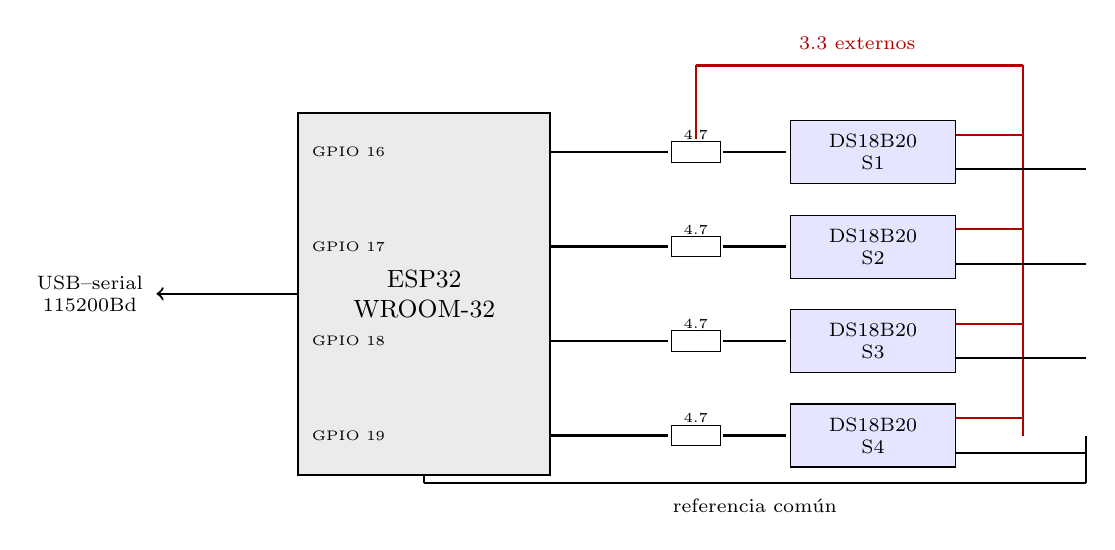
\begin{tikzpicture}[
      font=\small,
      mcu/.style   = {draw, thick, fill=black!8, minimum width=3.2cm,
                      minimum height=4.6cm, align=center},
      sensor/.style= {draw, fill=blue!10, minimum width=2.1cm,
                      minimum height=0.8cm, align=center, font=\scriptsize},
      res/.style   = {draw, fill=white, minimum width=0.62cm,
                      minimum height=0.26cm, inner sep=0pt,
                      font=\tiny},
      line/.style  = {thick}
    ]

    % --- microcontrolador -----------------------------------
    \node[mcu] (esp) at (0,0) {ESP32\\WROOM-32};

    % --- cuatro buses ---------------------------------------
    \foreach \i/\gpio/\y in {1/16/1.8, 2/17/0.6, 3/18/-0.6, 4/19/-1.8}{
      \node[anchor=west, font=\tiny] at (-1.55,\y) {GPIO \gpio};

      \draw[line] (1.6,\y) -- (3.1,\y);
      \node[res] (r\i) at (3.45,\y) {};
      \node[font=\tiny, above=1pt] at (r\i) {\SI{4.7}{\kilo\ohm}};
      \draw[line] (3.8,\y) -- (4.6,\y);

      \node[sensor] (s\i) at (5.7,\y) {DS18B20\\S\i};

      % pull-up hacia la línea de alimentación
      \draw[line] (r\i.north) ++(0,0) -- ++(0,0);
    }

    % --- línea de alimentación externa ----------------------
    \draw[line, red!70!black] (3.45,2.9) -- (7.6,2.9);
    \node[anchor=south, font=\scriptsize, text=red!70!black]
      at (5.5,2.98) {\SI{3.3}{\volt} externos};
    \draw[line, red!70!black] (3.45,2.9) -- (3.45,1.96);
    \foreach \y in {0.6, -0.6, -1.8}{
      \draw[line, red!70!black, opacity=0.6] (3.45,\y+0.16) -- (3.45,\y+0.16);
    }
    \draw[line, red!70!black] (7.6,2.9) -- (7.6,-1.8);
    \foreach \y in {1.8, 0.6, -0.6, -1.8}{
      \draw[line, red!70!black] (6.75,\y+0.22) -- (7.6,\y+0.22);
    }

    % --- referencia común -----------------------------------
    \draw[line] (0,-2.4) -- (8.4,-2.4);
    \node[anchor=north, font=\scriptsize] at (4.2,-2.48) {referencia común};
    \draw[line] (0,-2.3) -- (0,-2.4);
    \draw[line] (8.4,-2.4) -- (8.4,-1.8);
    \foreach \y in {1.8, 0.6, -0.6, -1.8}{
      \draw[line] (6.75,\y-0.22) -- (8.4,\y-0.22);
    }

    % --- enlace con la computadora --------------------------
    \draw[line, ->] (-1.6,0) -- (-3.4,0);
    \node[anchor=east, align=center, font=\scriptsize]
      at (-3.45,0) {USB--serial\\\SI{115200}{Bd}};

  \end{tikzpicture}}
  \caption{Módulo de medición de temperatura. Cada sensor DS18B20 ocupa
           un bus 1-Wire propio, con su resistencia de polarización y
           alimentación externa. La topología evita que el fallo de un
           dispositivo degrade la lectura de los restantes y hace que la
           línea afectada identifique al sensor.}
  \label{fig:modulo_temperatura}
\end{figure}
